\chapter{结果分析}

在预测结果方面可以发现预测结果与实际有些差别,这是因为预测糖尿病发展的模型还需要考虑到个体的生活方式、饮食习惯、锻炼频率等因素,因为这些因素可能随着时间的推移而改变. 例如,通过控制饮食、增加锻炼量等健康生活方式的改变,一个患有糖尿病前期的个体可能会改善其血糖水平,甚至避免糖尿病的发展. 因此,对于个体的血糖动力学模型的参数,需要进行实时调整以反映这些变化. 

并且同一个人在不同时间体内生产和消耗葡萄糖的速率也不是恒定的,如在睡眠状态时,体内大部分细胞活性都会降低,葡萄糖的生产和消耗速率都会降低,这时候进行模型拟合或者预测都是不准确的,再加上由于每个人体质不同,在进食后葡萄糖进入血液的速率也是未知的,因此选用清晨空腹时状态下的血糖数据进行模型拟合和预测是最为准确的. 这时候可以确保体内没有新的葡萄糖摄入,并且人体葡萄糖消耗速率也是正常水平. 

根据对二型糖尿病患者的数据分析,我们画出其血糖动力系统模型:
\begin{figure}[H]
    \centering
    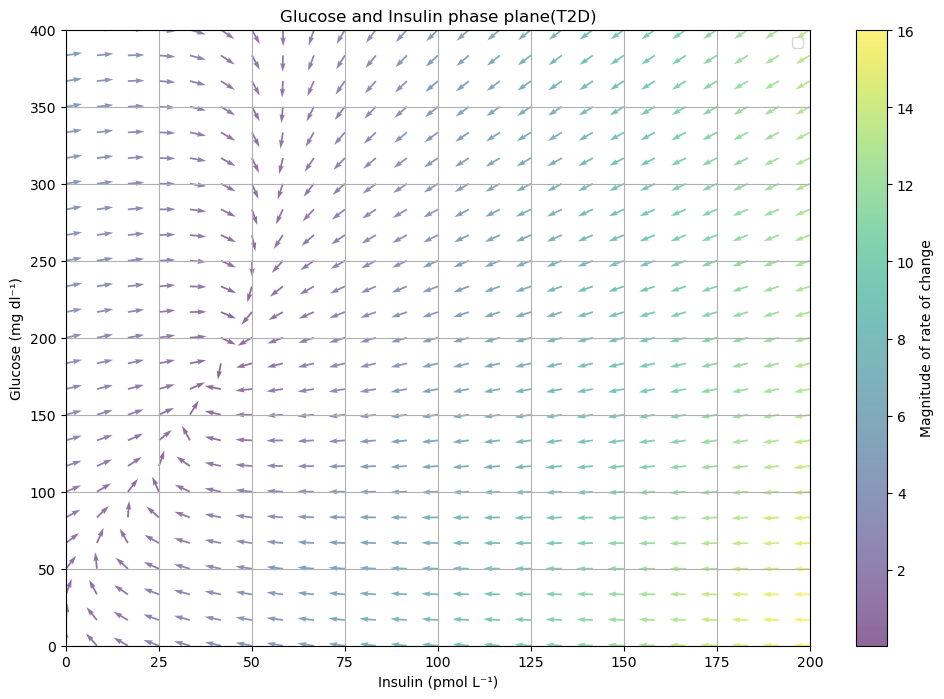
\includegraphics[width=0.8\textwidth]{Img/t2dphase.png}
    \bicaption{二型糖尿病患者血糖动力系统模型. }{Type 2 Diabetes patient blood glucose dynamic system model.}
    \label{fig:2type}
\end{figure}

对于正常人的血糖数据进行数据分析,我们画出其血糖动力系统模型:
\begin{figure}[H]
    \centering
    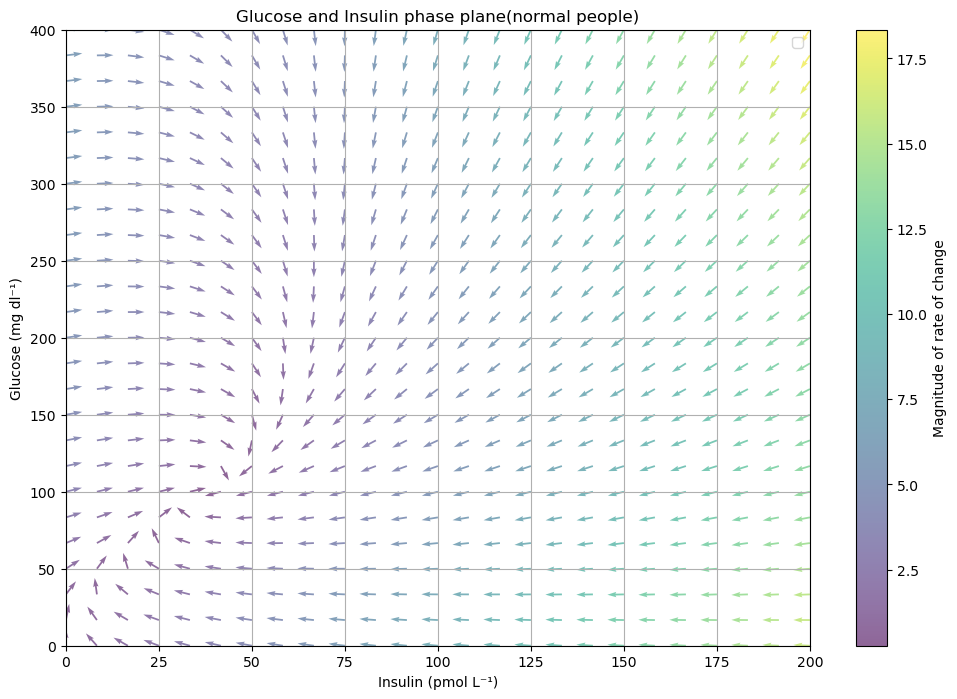
\includegraphics[width=0.8\textwidth]{Img/normalphase.png}
    \bicaption{正常人血糖动力系统模型. }{Normal person blood glucose dynamic system model.}
    \label{fig:normal}
\end{figure}

通过对比两者的模型,我们可以发现二型糖尿病患者的血糖动力系统模型与正常人的血糖动力系统模型并不相同. 再查看对应的模型参数我们可以发现二型糖尿病患者胰岛素敏感性这一参数显著低于正常人,这也是二型糖尿病患者与正常人的区别之处. 

而对于一型糖尿病患者的数据分析,我们画出其血糖动力系统模型:
\begin{figure}[H]
    \centering
    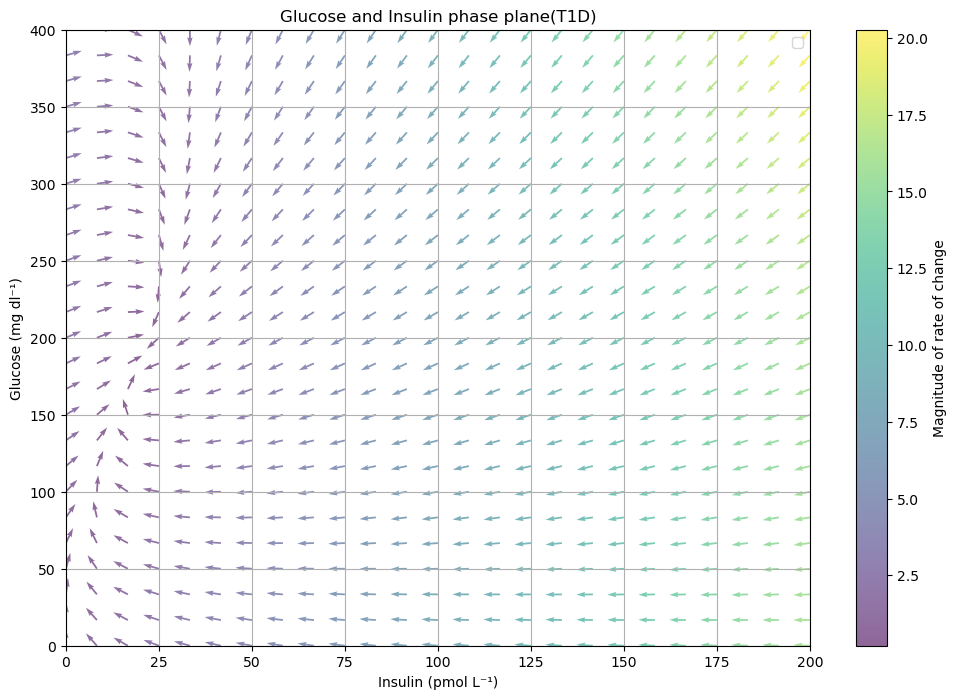
\includegraphics[width=0.8\textwidth]{Img/t1dphase.png}
    \bicaption{一型糖尿病患者血糖动力系统模型. }{Type 1 Diabetes patient blood glucose dynamic system model.}
    \label{fig:1type}
\end{figure}

通过对比一型糖尿病患者的血糖动力系统模型与正常人的血糖动力系统模型,可以发现一型糖尿病患者$b_1$这一参数显著低于正常人,也就是说这类患者要么胰$\beta$细胞数量较少,要么胰岛素分泌较慢,这也是一型糖尿病患者与正常人的区别之处. 

综上所述,对于通过连续血糖检测得到的血糖数据,我们可以通过模型\ref{model2}对其进行参数估计,得到其对应的血糖动力系统模型,通过对比其模型参数与正常值的范围,我们可以个性化的发现每个个体的状态,这也为糖尿病的治疗和管理提供了一定的参考. 

